%%=============================================================================
%% Conclusie
%%=============================================================================

\chapter{Conclusie}
\label{ch:conclusie}

% TODO: Trek een duidelijke conclusie, in de vorm van een antwoord op de
% onderzoeksvra(a)g(en). Wat was jouw bijdrage aan het onderzoeksdomein en
% hoe biedt dit meerwaarde aan het vakgebied/doelgroep? 
% Reflecteer kritisch over het resultaat. In Engelse teksten wordt deze sectie
% ``Discussion'' genoemd. Had je deze uitkomst verwacht? Zijn er zaken die nog
% niet duidelijk zijn?
% Heeft het onderzoek geleid tot nieuwe vragen die uitnodigen tot verder 
%onderzoek?

De onderzoeksvraag van deze bachelorproef luidde als volgt: `In welke mate kunnen AI's getraind worden om menselijke gevoelswaarden te herkennen in teksten?'. Deze vraag werd beantwoord door ten eerste twee externe tools zoals de Azure Text Analytics API en Google Cloud Platform te onderzoeken in hoofdstuk \ref{ch:methodologie}. Ten tweede werd ook een proof of concept gemaakt om op deze vraag te kunnen beantwoorden in hoofdstuk \ref{ch:proof-of-concept}. Deze bachelorproef onderzocht of AI sentimentele data kan halen uit reviews. Daarom werden er drie datasets gebruikt. Twee van deze dataset bevatten reviews en/of klachten die van de website zelf gehaald werden. Eén dataset bevatte tweets met reviews over vliegtuigmaatschappijen. Dit werd gedaan om variatie te creëren en zo een beter beeld te krijgen van de resultaten.

In welke mate kunnen AI's getraind worden om menselijke gevoelswaarden te herkennen in teksten? Natural Language Processing en Sentiment Analysis staan al heel ver. Er zijn verschillende tools en modellen die aan het vooraf bepaalde 80\% succespercentage voldoen. Google Cloud Platform bleek echter de beste resultaten te behalen.

Er waren ook een aantal deelvragen gedefinieerd. Deze zullen zo goed mogelijk beantwoord worden.

\section{Hoe ver staan Natural Language Processing en Sentiment Analysis al?}
\label{sec:hoever}
Op deze vraag kan duidelijk geantwoord worden dat NLP en Sentiment Analysis al heel ver staan. Zowel voor de externe tools, als voor de modellen werden er redelijk goede resultaten behaald op de drie datasets.
Voor alle modellen en externe tools werd ten minste een score van 75\% behaald. Dit betekent dat NLP en Sentiment Analysis al enorm gevorderd zijn.
In figuur \ref{fig:modellen} staan de modellen die in de proof of concept besproken werden. Het valt op dat alle modellen een redelijk goede score behaald hebben. Echter was model vier, wat een RNN (Recurrent Neural Netwerk) was, het beste model. Dit model voldeed wel aan de vooraf gedefinieerde 80\%.

\begin{figure}[!htbp]
    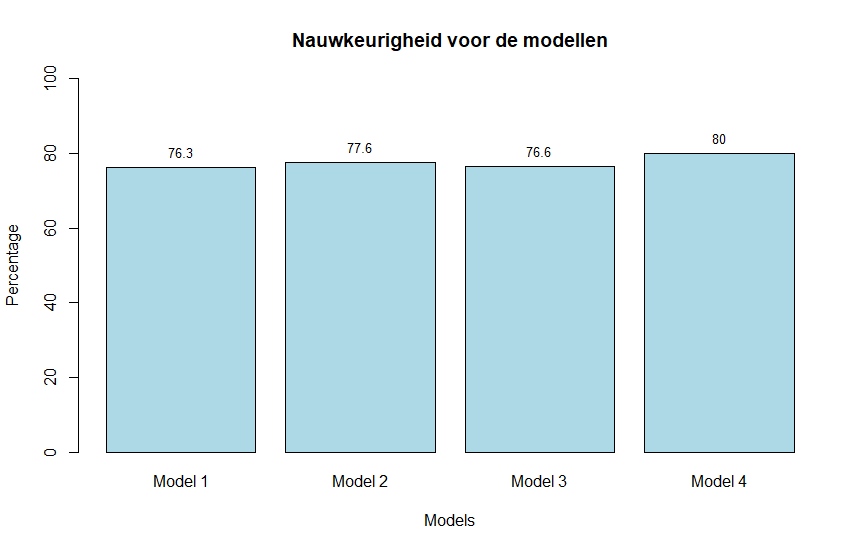
\includegraphics[width=\textwidth]{Grafieken/Modellen.PNG}
    \caption{\label{fig:modellen}Resultaten van alle modellen.}
\end{figure}
\FloatBarrier

In figuur \ref{fig:methodes} staat het beste model van de proof of concept in vergelijking met de twee externe methodes. Hier valt op dat Google Cloud Platform de beste gemiddelde resultaten opleverde. 

\begin{figure}[!htbp]
    \includegraphics[width=\textwidth]{Grafieken/methodes.PNG}
    \caption{\label{fig:methodes}Resultaten van alle methodes.}
\end{figure}
\FloatBarrier

Hieruit kan geconcludeerd worden dat NLP al heel ver staat, maar dat er nog ruimte is voor verbetering.

\section{Kunnen AI's bepaalde gevoelswaarden al begrijpen?}
\label{sec:gevoelswaarden}
Ja. Het is duidelijk dat AI's gemakkelijk het verschil tussen positieve, neutrale en negatieve reviews kunnen analyseren. Door de goede resultaten op de drie datasets, kan geconcludeerd worden dat NLP en AI's goed gevoelswaarden kunnen herkennen.

\section{Kunnen bedrijven Sentiment Analysis en Opinion Mining gebruiken bij het analyseren van hun reviews?}
\label{sec:reviews}
Het is enorm handig voor bedrijven om met de klant te kunnen communiceren aan de hand van gevoelswaarden die uit hun reviews afgeleid worden.
Het vooraf gedefinieerde succespercentage van 80\% werd bereikt. Daaruit kan besloten worden dat bedrijven dit zeker in de praktijk kunnen toepassen. Dit verhoogt immers de verstandshouding tussen het bedrijf en de klant.

\section{Verder Onderzoek}
\label{sec:verderonderzoek}
Natuurlijk is verder onderzoek nog vereist. Ten eerste zou het interessant zijn om verder onderzoek te doen naar hoe Artificiële Intelligentie gepast kan reageren op een review. Nu het duidelijk is dat AI gevoelswaarden uit een review kan afleiden, is verder onderzoek naar hoe men hierop reageert belangrijk. Verder kan er ook onderzoek gedaan worden naar modellen of methodes die een succespercentage van 90\% kunnen bereiken. Dit betekent meer zekerheid voor de bedrijven dat de AI juist reageert op de wensen van de klant.

